
\documentclass[10pt]{report}
%Packages
\usepackage{multirow}
\usepackage{graphicx}
\usepackage[utf8x]{inputenc}
\usepackage[T1]{fontenc}
\usepackage{aeguill}
\usepackage{amssymb}
\usepackage[french]{babel}
\usepackage{float}
\usepackage{fichetd}
\usepackage{mathenv}
\usepackage{tikz}
\usepackage[a4paper,pdftex=true]{geometry}
\usepackage{fancyvrb}

%Preamble

\input Cours/cqlsInclude
\input Cours/testInclude


\rightmargin -2cm
\leftmargin -1cm
\topmargin -2cm
\textheight 25cm

\newcommand{\redabr}{\textit{(rédaction abrégée) }}
\newcommand{\redstd}{\textit{(rédaction standard) }}

\setcounter{chapter}{4}
%Styles

%Title

\begin{document}



\chapter{Tests d'hypothèses}\label{TdHypo}
\noindent \fbox{\begin{minipage}{14.5cm}
\textbf{Avertissement~:} Dans la plupart des exercices ci-dessous traitant des tests d'hypothèses, les indications~\texttt{R} sont fournies à la fois pour le quantile et la p-valeur. Dans le cadre d'un examen, notez qu'un seul type d'indication~\texttt{R} est généralement fourni.
\end{minipage}}\\

\noindent \textbf{Quelques quantiles pour la loi $\mathcal{N}(0,1)$~:}
\begin{Verbatim}[frame=leftline,fontfamily=tt,fontshape=n,numbers=left]
> qnorm(c(0.8,0.9,0.95,0.975,0.99,0.995))
[1] 0.8416212 1.2815516 1.6448536 1.9599640 2.3263479 2.5758293
\end{Verbatim}


\bigskip

\begin{exercice}
Une certaine agence pour l'emploi affirme que le taux de
chômage en France serait cette année inférieur à $10\%$. Une
enquête auprès d'un échantillon de $200$ personnes choisies au hasard
dans la population active donne $16$ chômeurs.
\begin{enumerate}
\item Si on envisage un risque d'erreur de première 
espèce 
(maximal) 
fixé à 5\%, peut-on confirmer l'assertion avancée par l'agence.\\
\IndicR
\begin{Verbatim}[frame=leftline,fontfamily=tt,fontshape=n,numbers=left]
> 16/200
[1] 0.08
> # deltaEst.H0 <- (instruction R à fournir dans la rédaction)
> deltaEst.H0
[1] -0.942809
> pnorm(deltaEst.H0)
[1] 0.1728893
\end{Verbatim}

\item Peut-on pour autant montrer que l'agence pour 
l'emploi a effectué une mauvaise analyse?
 

\end{enumerate}
\end{exercice}

\begin{exercice} (suite du produit~A - Juin 2003)

Sur vos conseils, l'industriel a lanc{\'e} le produit A sur le march{\'e} (sa contrainte financi{\`e}re, rappelons-le, {\'e}tait de vendre mensuellement au moins 300000 exemplaires). Il est particuli{\`e}rement satisfait car d{\`e}s les deux premiers mois, il vend 350000 et 342000 exemplaires. Avec l'ambition qui le caract{\'e}rise, l'industriel souhaite am{\'e}liorer la qualit{\'e} de son produit car selon lui beaucoup de gens le connaissent alors que finalement peu l'ach{\`e}tent. Il estime que s'il parvient {\`a} montrer que plus de $80\%$ (strictement) des individus parmi la population cibl{\'e}e de taille $N=2000000$ connaissent le produit A (sans pour autant l'avoir achet{\'e}) alors il pourra investir dans l'am{\'e}lioration de son produit. Pour montrer ceci, il d{\'e}cide d'interroger au hasard $n=500$ individus (la question est moins ``grave'' que pour le lancement du produit A d'o{\`u} le choix d'un $n$ plus petit) issus de la population m{\`e}re. Les informations sont stock{\'e}es dans \texttt{R} dans le vecteur \texttt{yCA} (voir ci-apr{\`e}s). Sur cet {\'e}chantillon 420 personnes (autrement dit 84\% des individus interrog{\'e}s) lui ont r{\'e}pondu conna{\^\i}tre effectivement le produit~ A. \\
\begin{enumerate}
\item Pourriez-vous d{\'e}crire litt{\'e}ralement les deux erreurs mises en jeu dans cette probl{\'e}matique~? 



\item Peut-on montrer avec un risque d'erreur de premi{\`e}re esp{\`e}ce pr{\'e}fix{\'e} {\`a} 5\% que plus de 80\% (de gens parmi la population cibl{\'e}e) connaissent le produit~A~? Reportez sur le graphique ci-apr{\`e}s (repr{\'e}sentant la densit{\'e} d'une loi $\mathcal{N}(0,1)$) le quantile d'ordre 95\% ainsi que la p$-$valeur. 
 

\begin{center} 
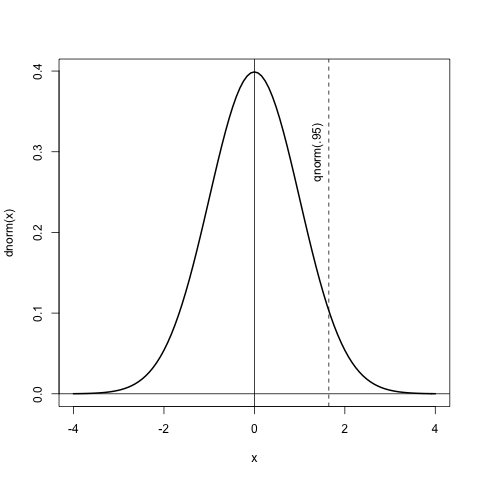
\includegraphics[scale=.45]{/Users/remy/Github/Statinf/Docus/td/img/N01corr.png}
\end{center}

\IndicR
\begin{Verbatim}[frame=leftline,fontfamily=tt,fontshape=n,numbers=left]
> yCA
  [1] 1 1 1 1 1 1 1 1 1 1 1 1 0 1 1 1 1 1 1 1 1 0 1 1 1 1 1 1 1 0 1 1 1 1 1 1 1
 [38] 1 1 0 1 1 0 1 0 1 1 1 1 1 1 1 0 1 1 1 1 1 1 1 1 1 1 1 1 1 1 1 1 1 1 1 1 0
...
[445] 1 1 1 1 0 1 1 1 1 1 1 1 0 1 1 1 1 0 1 1 1 1 1 1 1 1 1 0 1 1 1 1 1 1 1 1 1
[482] 1 0 0 1 1 1 1 1 0 1 1 1 1 0 1 1 0 1 1
> mean(yCA)
[1] 0.84
> # deltaEst.H0 <- (instruction R à fournir dans la rédaction)
> deltaEst.H0
[1] 2.236068
> pnorm(deltaEst.H0)
[1] 0.9873263
\end{Verbatim}



\item M{\^e}me question avec un risque d'erreur de premi{\`e}re esp{\`e}ce pr{\'e}fix{\'e} {\`a} 1\%~?




\end{enumerate}
\end{exercice}

\begin{exercice} (prime encouragement pour la qualité du produit A - contrôle continu 2003)

Comme chaque ann{\'e}e l'industriel afin d'encourager ses employ{\'e}s d{\'e}cide de leur verser une prime de fin d'ann{\'e}e si la client{\`e}le (potentielle) juge le produit~A de \textbf{bonne qualit{\'e}}. Sur une {\'e}chelle de valeurs  entre 0 et 10 mesurant le degr{\'e} de satisfaction, le produit est jug{\'e} de \textbf{bonne qualit{\'e}} si la note moyenne (sur les $N=2000000$ acheteurs potentiels), not{\'e}e $\mu^Q$, est strictement sup{\'e}rieure {\`a} 6 prouvant une qualit{\'e} plus qu'honorable de son produit.\\
\noindent \underline{Partie I (du point de vue de l'industriel)} (25 min.) \\

\begin{enumerate}
\item a) Exprimez l'assertion d'int{\'e}r{\^e}t conduisant {\`a} r{\'e}compenser les employ{\'e}s en fonction du param{\`e}tre d'int{\'e}r{\^e}t $\mu^Q$. \\



b) De quelles informations doit-on disposer pour {\'e}valuer le param{\`e}tre $\mu^Q$? Est-ce envisageable en pratique~?




Pour apporter un {\'e}l{\'e}ment de r{\'e}ponse, on d{\'e}cide d'interroger un {\'e}chantillon de 200 personnes. Chacun d'eux se prononce donc sur la qualit{\'e} du produit~A {\`a} travers une note de 0 {\`a} 10. En \texttt{R}, on stocke le jeu de donn{\'e}es $\Vect{y}^Q$ dans le vecteur \texttt{yQ}~:

\begin{Verbatim}[frame=leftline,fontfamily=tt,fontshape=n,numbers=left]
> yQ
  [1]  9  4  3  7  6  8  2  7  3  9  9  4  8  9  4  8 10  4  9  5  2  7  2  3  2
 [26]  4  9  6 10  8  5  5  5  5 10  7  4  4  4  4  6  8  2  8  9  5  7  8  6  4
...
[151]  7 10  6  5  4  9  5  6  4  2  6  7  5  6 10  8  6  5  9  7  2  2  2  8  9
[176]  6  3  8  7  6  3  8 10  2  2  8  9 10  9  8  2  7  7 10  3  3  2  9  7  6
\end{Verbatim}

 
\item a) D{\'e}crivez litt{\'e}ralement les deux erreurs de d{\'e}cision. 



b) Pr{\'e}cisez pour quelle(s) valeur(s) du param{\`e}tre d'int{\'e}r{\^e}t $\mu^Q$ inconnu chacune de ces deux erreurs intervient. 



c) Quelle vous semble {\^e}tre la plus grave de ces deux erreurs \textbf{du point de vue de l'industriel}~? 




d) A votre avis autour de quelles valeurs de $\mu^Q$ la d{\'e}cision vous semblera-t-elle difficile {\`a} prendre (cette valeur constituera la pire des situations)~? 





\item Dans la pire des situations (i.e. lorsque $\mu^Q=6$), la mesure d'{\'e}cart standardis{\'e}e de test s'{\'e}crit~: 
$$
\Est{\delta_{\mu^Q,6}}{Y^Q} = \frac{ \Est{\mu^Q}{Y^Q} - 6 }{ \sqrt{ \frac{\Est{\sigma_Q^2}{Y^Q}}{200}}} \SuitApprox \mathcal{N}(0,1)
$$
Rappeler tr{\`e}s bri{\`e}vement comment on peut interpr{\'e}ter ce r{\'e}sultat via l'Approche Exp{\'e}rimentale. 




\item a) Si on ne souhaite exc{\'e}der 5\% de risque de d{\'e}cider {\`a} tort de r{\'e}compenser les employ{\'e}s, {\'e}tablir la r{\`e}gle de d{\'e}cision et conclure quant {\`a} la bonne qualit{\'e} du produit en vous aidant des quelques instructions \texttt{R}. \\
b) Concr{\`e}tement, quelle d{\'e}cision doit prendre l'industriel quant au versement de la prime de fin d'ann{\'e}e.

\IndicR
\begin{Verbatim}[frame=leftline,fontfamily=tt,fontshape=n,numbers=left]
> mean(yQ)
[1] 6.245
> sd(yQ)
[1] 2.458699
> # deltaEst.H0 <- (instruction R à fournir dans la rédaction)
> deltaEst.H0
[1] 1.40921
> pnorm(deltaEst.H0)
[1] 0.9206135
\end{Verbatim}

 



\end{enumerate}

\noindent \underline{Partie II (du point de vue des employ{\'e}s)} (25 min.) \\

Ind{\'e}pendamment des r{\'e}ponses pr{\'e}c{\'e}dentes un employ{\'e} ayant de solides connaissances en statistiques s'interroge sur le test pr{\'e}c{\'e}dent et notamment sur les deux risques d'erreur de d{\'e}cision mis en jeu. 

\begin{enumerate}
\item \textbf{Du point de vue des employ{\'e}s}, quelle est la plus grave des deux erreurs de d{\'e}cision dans le test pr{\'e}c{\'e}dent~?



\item En tant que d{\'e}l{\'e}gu{\'e}, un employé exprime alors au nom de ses coll{\`e}gues la revendication suivante~: ``nous acceptons de ne pas recevoir de prime de fin d'ann{\'e}e si vous pouvez prouver au vu du m{\^e}me jeu de donn{\'e}es pr{\'e}c{\'e}dent que le produit n'est pas de bonne qualit{\'e} (i.e. $\mu^Q<6$)''. Peut-on prouver au vu des donn{\'e}es que la note moyenne du degr{\'e} de satisfaction est strictement inf{\'e}rieure {\`a} 6~? (Indication~: r{\'e}daction standard et conclure en fournissant la valeur de la p$-$valeur)
 

\item Ce d{\'e}l{\'e}gu{\'e} d{\'e}sireux d'approfondir son argumentation, pose la question suivante {\`a} l'industriel~: ``si on avait obtenu $\Est{\mu^Q}{y^Q}$ et $\Est{\sigma_{Q}}{y^Q}$ de l'ordre de 6.245 et 2.459 respectivement non pas avec la taille d'{\'e}chantillon actuelle de $n=200$ mais avec une taille plus grande, pensez-vous que vous auriez pu montrer que le produit {\'e}tait de bonne qualit{\'e}~?''\\
Et vous qu'en pensez-vous en vous aidant des instructions suivantes (en particulier si la taille d'{\'e}chantillon avait {\'e}t{\'e} $n=300$, $n=500$ et $n=1000$)~?

\begin{Verbatim}[frame=leftline,fontfamily=tt,fontshape=n,numbers=left]
> (mean(yQ)-6)/sqrt(var(yQ)/300)
[1] 1.725923
> pnorm((mean(yQ)-6)/sqrt(var(yQ)/1000))
[1] 0.9991867
\end{Verbatim}


 
\end{enumerate}
\end{exercice}

\begin{exercice} (compétence)
Un service de contr{\^o}le d'une entreprise de m{\'e}tallurgie s'int{\'e}resse {\`a} savoir si un technicien est suffisamment pr{\'e}cis au niveau des mesures quotidiennes qu'il effectue sur des minerais de fer (les mesures effectu{\'e}es sont des mesures de diam{\`e}tre). Une comp{\'e}tence ``suffisante'' que nous allons d{\'e}finir) sera r{\'e}compens{\'e}e par une prime. Le technicien sera d'autant plus précis que l'écart entre deux mesures d'un même minerai (sans qu'il le sache) est faible. Fort de constater que l'écart moyen est théoriquement nul (à justifier), la précision sera naturellement mesurée  par la variance des écarts. 

Soit $Y^C$  un futur écart entre deux mesures d'un même minerai. C'est une variable aléatoire qui est caractérisée (via l'approche expérimentale) par la donnée d'une infinité d'écarts virtuels (entre deux mesures) $y^C_{[1]},\ldots,y^C_{[m]},\ldots$. On notera $\sigma^2_C$ la variance de l'infinité de ces écarts de mesure qui constitue l'indicateur du niveau de précision du technicien. Cet indicateur  constitue le param{\`e}tre d'int{\'e}r{\^e}t de l'{\'e}tude. Le service de contr{\^o}le d{\'e}cide que le technicien est comp{\'e}tent (et pourra ainsi lui verser une prime) si le param{\`e}tre d'int{\'e}r{\^e}t est inf{\'e}rieur {\`a} $0.1$. \\

\begin{enumerate}

\item Au vu des données peut-on montrer que le technicien est compétent avec un risque d'erreur de première espèce fixé à 5\%.

\IndicR
\begin{Verbatim}[frame=leftline,fontfamily=tt,fontshape=n,numbers=left]
> yC
 [1]  0.34520624  0.36187714  0.28326083 -0.04273267  0.07897429 -0.57583456
 [7] -0.71994324  0.18188198  0.04438047 -0.01951828 -0.34820050  0.26067820
...
[25]  0.31212572  0.12692537 -0.17803505 -0.17861634 -0.48143225 -0.07185419
> var(yC)
[1] 0.08843689
> # deltaEst.H0 <- (instruction R à fournir dans la rédaction)
> deltaEst.H0
[1] -0.5474076
> pnorm(deltaEst.H0)
[1] 0.2920494
\end{Verbatim}

 


\item Le service de contr{\^o}le ({\`a} qui on a fait comprendre que le risque $\alpha$ est g{\'e}n{\'e}ralement fix{\'e} {\`a} $5\%$) d{\'e}cide au vu de la p-valeur du pr{\'e}c{\'e}dent test de renvoyer sur le champ le technicien. Ce dernier bien plus au courant des techniques statistiques assigne son employeur aux prud'hommes et gagne le proc{\`e}s haut la main. L'argument avanc{\'e} par le technicien est le suivant : ``Le service de contr{\^o}le n'a en aucun cas prouv{\'e} que je n'{\'e}tais pas comp{\'e}tent. Il n'a seulement pas pu prouver au vu des donn{\'e}es que j'{\'e}tais comp{\'e}tent : soit il prouve que je ne suis pas comp{\'e}tent, soit il me soumet {\`a} un nombre plus {\'e}lev{\'e} d'{\'e}chantillons de mani{\`e}re {\`a} ce que l'estimation de la variance soit significative.''. Essayez de traduire math{\'e}matiquement l'argument du technicien. 



\item Le service de contr{\^o}le d{\'e}cide alors de soumettre deux fois le technicien {\`a} $n=500$ mesures sur les {\'e}chantillons de minerai. Le vecteur des 500 {\'e}carts de mesures est encore not{\'e} ${\bf y}^C$. Avec ces nouvelles observations que concluez-vous au seuil de $5 \%$ ? \\

\IndicR
\begin{Verbatim}[frame=leftline,fontfamily=tt,fontshape=n,numbers=left]
> yC
  [1]  0.345206239  0.361877141  0.283260829 -0.042732674  0.078974292
  [6] -0.575834563 -0.719943239  0.181881984  0.044380473 -0.019518279
...
[491] -0.070185269  0.134088213  0.277789013 -0.079484256 -0.107560964
[496] -0.265767699 -0.124663757 -0.026684338  0.494449721 -0.304572345
> var(yC)
[1] 0.08299474
> # deltaEst.H0 <- (instruction R à fournir dans la rédaction)
> deltaEst.H0
[1] -3.299262
> pnorm(deltaEst.H0)
[1] 0.0004846965
\end{Verbatim}

 

\end{enumerate}
\end{exercice}

\begin{exercice}(diététicien)
Un di{\'e}t{\'e}ticien affirme que son r{\'e}gime alimentaire permet une perte de poids rapide. On observe la r{\'e}partition d'un {\'e}chantillon de $10$ femmes ayant suivi ce r{\'e}gime pendant $2$ semaines.
$$
\begin{tabular}{|c|c|c|c|c|c|c|c|c|c|c|}\hline
{\bf Poids avant AV} &
$64$ & $67$ & $68$ & $76$ & $72$ & $69$ & $62$ & $65$ & $64$ & $73$ \\\hline
{\bf Poids apr{\`e}s AP} &
$65$ & $61$ & $64$ & $69$ & $65$ & $66$ & $60$ & $59$ & $61$ & $68$ \\\hline
{\bf Perte de poids $Y$} &
$-1$ & $6$ & $4$ & $7$ & $7$ & $3$ & $2$ & $6$ & $3$ & $5$ \\\hline
\end{tabular}
$$

\textit{Voici les donn{\'e}es pr{\'e}liminairement saisies et plac{\'e}es dans deux vecteurs $\Vect{AV}$ et $\Vect{AP}$. Le vecteur $\Vect{y}$ est obtenu en faisant une diff{\'e}rence {\'e}l{\'e}ment par {\'e}l{\'e}ment}~:

\IndicR
\begin{Verbatim}[frame=leftline,fontfamily=tt,fontshape=n,numbers=left]
> AV-AP
 [1] -1  6  4  7  7  3  2  6  3  5
> mean(AV-AP)
[1] 4.2
> sd(AV-AP)
[1] 2.529822
> seMean(AV-AP)
[1] 0.8
\end{Verbatim}


1. En supposant que $Y\leadsto N\left( \mu ,\sigma \right) $, {\'e}prouver
l'affirmation du di{\'e} t{\'e}ticien au seuil de signification $5\%$.

\IndicR
\begin{Verbatim}[frame=leftline,fontfamily=tt,fontshape=n,numbers=left]
> # deltaEst.H0 <- (instruction R à fournir dans la rédaction)
> deltaEst.H0
[1] 5.25
> pt(deltaEst.H0,9)
[1] 0.9997362
\end{Verbatim}



2. Fort de ce constat, le di{\'e}t{\'e}ticien aimerait un titre plus accrocheur et souhaiterait montrer avec le m{\^e}me jeu de donn{\'e}es $\Vect{y}$ que son r{\'e}gime permet une perte de deux kilos par semaine. {\'E}prouvez cette nouvelle affirmation au seuil de 5\%.

\IndicR
\begin{Verbatim}[frame=leftline,fontfamily=tt,fontshape=n,numbers=left]
> # deltaEst.H0 <- (instruction R à fournir dans la rédaction)
> deltaEst.H0
[1] 0.25
> pt(deltaEst.H0,9)
[1] 0.5958998
\end{Verbatim}




3. Pas d{\'e}sappoint{\'e} pour autant par la pr{\'e}c{\'e}dente analyse, le di{\'e}t{\'e}ticien d{\'e}cide de soumettre 40 femmes suppl{\'e}mentaires {\`a} son r{\'e}gime, et compl{\`e}te ainsi son pr{\'e}c{\'e}dent vecteur $\Vect{y}$ correspondant aux pertes de poids. Il obtient finalement le jeu de donn{\'e}es suivant~:

\IndicR
\begin{Verbatim}[frame=leftline,fontfamily=tt,fontshape=n,numbers=left]
> yD
 [1] -1  6  4  7  7  3  2  6  3  5  5  7  4  4  2  4  6  6  5  3  5  5  2  7  4
[26]  5  4  3  6  7  4  6  4  5  2  6  4  6  5  5  6  4  3  2  3  6  5  7  2  4
> mean(yD)
[1] 4.5
> sd(yD)
[1] 1.729103
> seMean(yD)
[1] 0.244532
\end{Verbatim}
 
 
a) que pensez-vous alors de l'hypoth{\`e}se faite pr{\'e}c{\'e}demment affirmant~: $Y\leadsto N\left( \mu ,\sigma \right) $~?



b) pensez-vous avec ce nouveau jeu de donn{\'e}es que la nouvelle affirmation du di{\'e}t{\'e}ticien est vraie ({\`a} un risque d'erreur de premi{\`e}re esp{\`e}ce fix{\'e} {\`a} 5\%)~?

\IndicR
\begin{Verbatim}[frame=leftline,fontfamily=tt,fontshape=n,numbers=left]
> # deltaEst.H0 <- (instruction R à fournir dans la rédaction)
> deltaEst.H0
[1] 2.044722
> pnorm(deltaEst.H0)
[1] 0.9795589
\end{Verbatim}




c) Qu'expriment les erreurs standard (\texttt{seMean(y)}) pour $n=10$ et $n=50$~? Expliquez alors pourquoi on a pu accepter l'assertion d'intérêt du diététicien pour $n=50$.


\end{exercice}

\begin{exercice}

Un pilote de course en Formule 1 hésite entre deux équipes. Il fait alors des essais dans chacune des deux équipes pour savoir laquelle est la plus performante.\\

\noindent 1) Pour l'équipe 1, le pilote commence par faire 20 premiers tours. Les données des temps effectués par tour sont exprimées en secondes et stockées dans le vecteur  \texttt{y1}. Au vu des données peut-on montrer que le temps moyen de la voiture de l'équipe 1 est inférieur à 51 secondes  avec un risque d'erreur de première espèce fixé à 5\%~?\\

\IndicR
\begin{Verbatim}[frame=leftline,fontfamily=tt,fontshape=n,numbers=left]
> mean(y1)
[1] 50.21973
> sd(y1)
[1] 2.276776
> # deltaEst.H0 <- (instruction R à fournir dans la rédaction)
> deltaEst.H0
[1] -1.532634
> pt(deltaEst.H0,19)
[1] 0.07092418
\end{Verbatim}




\noindent 2) Le pilote effectue 20 tours supplémentaires (les données sont toujours stockées dans le vecteur \texttt{y1}).
Même question que précédemment avec ce nouveau jeu de données complétées.\\
\IndicR
\begin{Verbatim}[frame=leftline,fontfamily=tt,fontshape=n,numbers=left]
> y1
 [1] 47.89674 50.04087 54.53240 54.36718 48.80645 51.44077 49.72669 44.81843
 [9] 50.37910 48.32037 53.55150 50.38611 50.37899 49.44585 50.47262 50.66881
...
[33] 48.83423 51.93978 49.19886 52.67034 49.21360 48.35678 49.43116 48.95199
> mean(y1)
[1] 50.39458
> sd(y1)
[1] 1.965069
> # deltaEst.H0 <- (instruction R à fournir dans la rédaction)
> deltaEst.H0
[1] -1.948534
> pnorm(deltaEst.H0)
[1] 0.02567557
\end{Verbatim}




\noindent 3) Avec la voiture de l'équipe~2,  le pilote effectue 50 tours. Les données des temps effectués par tour sont exprimées en secondes et stockées dans le vecteur  \texttt{y2}. Au vu des données peut-on montrer que le temps moyen de la voiture de l'équipe 2 est inférieur à 51 secondes  avec un risque d'erreur de première espèce fixé à 5\%~?\\

\IndicR
\begin{Verbatim}[frame=leftline,fontfamily=tt,fontshape=n,numbers=left]
> y2
 [1] 51.89371 51.35814 52.16305 51.83228 52.97653 51.43513 50.89370 51.50756
 [9] 51.54468 52.22917 51.21122 52.96252 51.61797 52.40225 50.21097 51.73468
...
[49] 53.55974 52.44708
> mean(y2)
[1] 52.02422
> sd(y2)
[1] 0.8670206
> # deltaEst.H0 <- (instruction R à fournir dans la rédaction)
> deltaEst.H0
[1] 8.353126
> pnorm(deltaEst.H0)
[1] 1
\end{Verbatim}




\noindent 4) Quel est l'ordre de grandeur de la p$-$valeur du précédent test~? Donc à la vue des sorties R précédentes, les données permettent-elles de laisser penser qu'une certaine assertion d'intérêt (à préciser) est vraie~?



\noindent 5) Au vu des données peut-on montrer que le temps moyen de l'équipe~1 est inférieur à celui de l'équipe~2  avec un risque d'erreur de première espèce fixé à 5\%~?\\
Cela est-il surprenant au regard le la conclusion de la question précédente~?\\
\IndicR
\begin{Verbatim}[frame=leftline,fontfamily=tt,fontshape=n,numbers=left]
> # deltaEst.H0 <- (instruction R à fournir dans la rédaction)
> deltaEst.H0
[1] -4.878811
\end{Verbatim}




\noindent 6) Au vu des données peut-on montrer que la variance des temps de l'équipe~2 est inférieure à celle de l'équipe~1  avec un risque d'erreur de première espèce fixé à 5\%~?\\
\IndicR
\begin{Verbatim}[frame=leftline,fontfamily=tt,fontshape=n,numbers=left]
> # deltaEst.H0 <- (instruction R à fournir dans la rédaction)
> deltaEst.H0
[1] 3.161661
\end{Verbatim}




\noindent 7) Exprimez littéralement les deux conclusions des deux tests précédents. Si vous étiez le pilote, quelle équipe choisiriez-vous~?



\end{exercice}

\begin{exercice} (1h - environ 10 pts)

\noindent \underline{Partie I: compétence d'un technicien} \\

Un service de contr{\^o}le d'une entreprise de m{\'e}tallurgie s'int{\'e}resse {\`a} savoir si un technicien (Alfred) est suffisamment pr{\'e}cis au niveau des mesures qu'il effectue sur des minerais de fer. Le technicien sera d'autant plus précis que l'écart entre deux mesures d'un même minerai (sans qu'il le sache) est faible. La précision serait théoriquement mesurée  par la variance d'une infinité d'écarts entre deux mesures. On notera $\sigma^2_A$ (comme Alfred) cette variance.  Le service de contr{\^o}le d{\'e}cide qu'un technicien est comp{\'e}tent si ce param{\`e}tre d'int{\'e}r{\^e}t est inf{\'e}rieur {\`a} $0.1$. \\ 

\begin{enumerate}
\item On commence par soumettre Alfred à $n^A=20$ échantillons de minerai de fer. Le jeu de données est stocké dans le vecteur \texttt{yA} dans \texttt{R}. Peut-on montrer au seuil de $5\%$ qu'Alfred est compétent~? (précisez l'hypothèse mathématique faite sur la nature des données)

\IndicR
\begin{Verbatim}[frame=leftline,fontfamily=tt,fontshape=n,numbers=left]
> yA
 [1]  0.14467956  0.30839102  0.16507184  0.08100885 -0.15048984 -0.02163446
 [7] -0.25558794  0.09871536  0.59275135 -0.22962500 -0.21676732 -0.09707208
[13]  0.17050529 -0.05732366  0.65337514  0.17802469  0.29278735 -0.16514972
[19] -0.30080221  0.32129752
> var(yA)
[1] 0.07325571
> sd(yA)
[1] 0.2706579
> # deltaEst.H0 <- (instruction R à fournir dans la rédaction)
> deltaEst.H0
[1] 13.91858
> qchisq(c(0.01,0.025,0.05,0.1,0.9,0.95,0.975,0.99),19)
[1]  7.632730  8.906516 10.117013 11.650910 27.203571 30.143527 32.852327
[8] 36.190869
> pchisq(deltaEst.H0,19)
[1] 0.2115835
\end{Verbatim}




\item On complète le jeu de données précédent en soumettant le technicien à 30 \textbf{nouveaux} échantillons. Le jeu de données est toujours stocké dans le vecteur \texttt{yA}. Peut-on maintenant montrer au seuil de $5\%$ que le technicien est compétent~?

\IndicR
\begin{Verbatim}[frame=leftline,fontfamily=tt,fontshape=n,numbers=left]
> yA
 [1]  0.144679564  0.308391020  0.165071844  0.081008851 -0.150489836
 [6] -0.021634458 -0.255587943  0.098715356  0.592751352 -0.229624997
...
[41]  0.262084534 -0.215753300  0.173626815 -0.200160681 -0.255138748
[46]  0.125329351 -0.326049545  0.207517750  0.070438920 -0.303221493
> var(yA)
[1] 0.06362229
> sd(yA)
[1] 0.2522346
> # deltaEst.H0 <- (instruction R à fournir dans la rédaction)
> deltaEst.H0
[1] -2.762438
> pnorm(deltaEst.H0)
[1] 0.002868572
\end{Verbatim}



\end{enumerate}

\noindent \underline{Partie II : comparaison de deux techniciens} \\

\begin{enumerate}

\item On s'intéresse à un second technicien (Bernard) dont on cherche à montrer qu'il est compétent. Bernard a été soumis à $n^B=20$ échantillons de minerai; les données relatives à ses écarts de mesure sont stockées en \texttt{R} dans le vecteur \texttt{yB}. Peut-on montrer qu'il est compétent au seuil de 5\%~?


\IndicR
\begin{Verbatim}[frame=leftline,fontfamily=tt,fontshape=n,numbers=left]
> yB
 [1]  0.024830162  0.093791329  0.145188006 -0.049699994 -0.153214255
 [6]  0.120875740 -0.112933043 -0.345291716 -0.007106278  0.122016115
[11] -0.191976511 -0.368424436  0.188209329 -0.119061948 -0.202052804
[16]  0.249518927 -0.301396393  0.112303313  0.216480111  0.239335084
> var(yB)
[1] 0.03921612
> # deltaEst.H0 <- (instruction R à fournir dans la rédaction)
> deltaEst.H0
[1] 7.451062
\end{Verbatim}




\item Peut-on montrer (toujours au seuil de 5\%) qu'Alfred est moins précis que Bernard~?


\IndicR
\begin{Verbatim}[frame=leftline,fontfamily=tt,fontshape=n,numbers=left]
> # deltaEst.H0 <- (instruction R à fournir dans la rédaction)
> deltaEst.H0
[1] 1.622351
> qf(c(0.01,0.025,0.05,0.1,0.9,0.95,0.975,0.99),49,19)
[1] 0.4350385 0.4954826 0.5546675 0.6325832 1.7129041 2.0008646 2.2983466
[8] 2.7135032
\end{Verbatim}





\item Alfred et Bernard critiquent le précédent résultat et proposent de refaire le même test à taille d'échantillon identique (i.e. $n=20$). Que peut-on dire à la vue de l'instruction ci-dessous~?

\IndicR
\begin{Verbatim}[frame=leftline,fontfamily=tt,fontshape=n,numbers=left]
> # deltaEst.H0 <- (instruction R à fournir dans la rédaction)
> pf(deltaEst.H0,19,19)
[1] 0.9088193
\end{Verbatim}




\item On complète alors le jeu de données du second technicien, en soumettant Bernard à 40 \textbf{nouveaux} échantillons (les données sont toujours stockées en \texttt{R} dans le vecteur \texttt{yB}). Peut-on cette fois-ci montrer qu'Alfred est moins précis que Bernard~?

\IndicR
\begin{Verbatim}[frame=leftline,fontfamily=tt,fontshape=n,numbers=left]
> yB
 [1]  0.024830162  0.093791329  0.145188006 -0.049699994 -0.153214255
 [6]  0.120875740 -0.112933043 -0.345291716 -0.007106278  0.122016115
...
[51]  0.296275243 -0.162141374  0.060792874  0.090976915  0.119856496
[56]  0.310565975 -0.146785494  0.061968269 -0.182127778 -0.187890277
> var(yB)
[1] 0.03442929
> # deltaEst.H0 <- (instruction R à fournir dans la rédaction)
> deltaEst.H0
[1] 2.037317
\end{Verbatim}




\end{enumerate}
\end{exercice}

\begin{exercice} (conduite)

Un exp{\'e}rimentateur veut savoir si les femmes conduisent mieux que les
hommes au vu des notes de conduite suivantes~:
 
{\bf Hommes} : 24,28,29,29,34,36,40,41 et 60.

{\bf Femmes }: 21,31,34,37,38,39,42,43,44,50 et 51.

Nous supposerons que $Y^{H}\leadsto N\left( \mu^{H} ,\sigma_{H} \right) $ et $Y^{F}\leadsto N\left( \mu^{F},\sigma_{F} \right) $, et nous choisirons un seuil de signification de $5\%$.


\IndicR
\begin{Verbatim}[frame=leftline,fontfamily=tt,fontshape=n,numbers=left]
> yH
[1] 24 28 29 29 34 36 40 41 60

> yF
 [1] 21 31 34 37 38 39 42 43 44 50 51
> mean(yH)
[1] 35.66667
> mean(yF)
[1] 39.09091
> sd(yH)
[1] 10.75872
> sd(yF)
[1] 8.561011
> # deltaEst.H0 <- (instruction R à fournir dans la rédaction)
> deltaEst.H0
[1] -0.7935825
> pt(deltaEst.H0,18)
[1] 0.2188878
\end{Verbatim}




Traitement hors exercice pour v{\'e}rifier si l'hypoth{\`e}se sur l'{\'e}galit{\'e} des variances de X et Y n'{\'e}tait pas abusive~:

\IndicR
\begin{Verbatim}[frame=leftline,fontfamily=tt,fontshape=n,numbers=left]
> # deltaEst.H0 <- (instruction R à fournir dans la rédaction)
> deltaEst.H0
[1] 1.579323
> pf(deltaEst.H0,8,10)
[1] 0.7550565
\end{Verbatim}




\end{exercice}

\begin{exercice}

Situons le contexte  de cette étude pour laquelle toute ressemblance avec une situation ou des personnages ayant réellement existé serait purement fortuite : nous sommes un peu \textbf{avant le premier tour} des élections présidentielles de 2001. Parmi l'ensemble des candidats, nous nous intéresserons aux trois principaux~: Racchi, Pinjos et Penle.  On notera dans l'ordre $p^{C1}$, $p^{C2}$ et $p^{C3}$ les proportions d'électeurs (parmi tout l'électorat) ayant voté pour ces trois candidats.

Un journaliste interroge ces trois candidats séparément et leur demande le score que chacun pense faire au premier tour. Racchi pense réaliser un score autour de 20\%, Pinjos autour de 19\% et Penle 18\%.  Le journaliste n'ayant pas confiance sur la façon dont sont construits les sondages se crée un échantillon de $n=1000$ (choisis au hasard dans l'électorat français) et obtient les trois estimations $\Est{p^{C1}}{y}=20\%$, $\Est{p^{C2}}{y}=15.4\%$ et $\Est{p^{C3}}{y}=18.3\%$ stockés en \texttt{R} respectivement dans les variables \texttt{pC1Est}, \texttt{pC2Est} et \texttt{pC3Est}.

\begin{enumerate}
\item Au vu des a priori des trois candidats et de ce que semblent penser les médias et la population,  le journaliste veut alors savoir si la proportion d'électeurs votant pour
\begin{itemize}
\item[a)] Racchi est au moins de 17.5\%.
\item[b)] Pinjos est au moins de 17.5 \%.
\item[c)] Penle est inférieure à 17.5 \%.
\end{itemize} 
Formez les trois tests d'hypothèses répondant à ces questions pour un risque d'erreur de première espèce qui n'excède pas 5\%.  Rédigez sous forme standard le premier test. 

\IndicR
\begin{Verbatim}[frame=leftline,fontfamily=tt,fontshape=n,numbers=left]
> 200/1000
[1] 0.2
> # deltaEst.H0 <- (instruction R à fournir dans la rédaction)
> deltaEst.H0
[1] 2.080626
> pnorm(deltaEst.H0)
[1] 0.9812659
\end{Verbatim}

\begin{Verbatim}[frame=leftline,fontfamily=tt,fontshape=n,numbers=left]
> 154/1000
[1] 0.154
> # deltaEst.H0 <- (instruction R à fournir dans la rédaction)
> deltaEst.H0
[1] -1.747726
> pnorm(deltaEst.H0)
[1] 0.04025576
\end{Verbatim}

\begin{Verbatim}[frame=leftline,fontfamily=tt,fontshape=n,numbers=left]
> 183/1000
[1] 0.183
> # deltaEst.H0 <- (instruction R à fournir dans la rédaction)
> deltaEst.H0
[1] 0.6658003
> pnorm(deltaEst.H0)
[1] 0.7472306
\end{Verbatim}




\item Pour les candidats Pinjos et Penle (qui ne sont pas sur un bateau) peut-on montrer le contraire des assertions respectives (justifiez en rédigeant succinctement)~?


\item La situation semblant plus préoccupante pour Pinjos et Penle, le journaliste tente de les départager en proposant de vérifier à partir du même jeu de données les assertions suivantes mais au seuil de $\alpha=20\%$ (réponse sous la forme de rédaction abrégée)~:
\begin{itemize}
\item[a)] le score de Pinjos est inférieur à 16.5\%
\item[b)] le score de Penle est supérieur à 16.5\%
\end{itemize}






\IndicR
\begin{Verbatim}[frame=leftline,fontfamily=tt,fontshape=n,numbers=left]
> 154/1000
[1] 0.154
> # deltaEst.H0 <- (instruction R à fournir dans la rédaction)
> deltaEst.H0
[1] -0.9371465
\end{Verbatim}

\begin{Verbatim}[frame=leftline,fontfamily=tt,fontshape=n,numbers=left]
> 183/1000
[1] 0.183
> # deltaEst.H0 <- (instruction R à fournir dans la rédaction)
> deltaEst.H0
[1] 1.533512
\end{Verbatim}





\end{enumerate}

\end{exercice}

\begin{exercice} (rapport adjectifs-verbe)

Un psychologue est intéressé par le rapport adjectif-verbe pour caractériser le style de discours d'un individu. Il veut alors savoir s'il y a une différence de style entre les étudiants. Un échantillon de 10 étudiants de chaque formation est choisi. Chque étudiant écrit un ensemble de textes libres. Le rapport entre le nombre de verbes et le nombre d'adjectifs utilisés par chaque est étudiant est donné dans le tableau suivant~:

\begin{tabular}{|l|cccccccccc|}
\hline
scientifique&1.04& 0.93& 0.75& 0.33& 1.62& 0.76& 0.97& 1.21& 0.8 &1.18 \\
litteraire& 1.32& 2.3 & 1.98 &0.59& 1.02 &0.88& 0.92& 1.39 &1.95 &1.25 \\
\hline
\end{tabular}

1) Peut-on plutôt penser que les scientifiques d'une part et les littéraires d'autre part utilisent plus de deux fois plus d'adjectifs que de verbes~?

\IndicR
\begin{Verbatim}[frame=leftline,fontfamily=tt,fontshape=n,numbers=left]
> sc
 [1] 1.04 0.93 0.75 0.33 1.62 0.76 0.97 1.21 0.80 1.18
> mean(sc)
[1] 0.959
> sd(sc)
[1] 0.343267
> deltaEst.H0
[1] 4.228445
> pt(deltaEst.H0,9)
[1] 0.9988942
\end{Verbatim}
 
\begin{Verbatim}[frame=leftline,fontfamily=tt,fontshape=n,numbers=left]
> litt
 [1] 1.32 2.30 1.98 0.59 1.02 0.88 0.92 1.39 1.95 1.25
> mean(litt)
[1] 1.36
> sd(litt)
[1] 0.5540959
> deltaEst.H0
[1] 4.908102
> pt(deltaEst.H0,9)
[1] 0.9995809
\end{Verbatim}
 
 


2) Peut-on penser que le discours des littéraires est plus littéraire que celui des scientifiques avec un risque d'erreur de 5\%~?

\IndicR
\begin{Verbatim}[frame=leftline,fontfamily=tt,fontshape=n,numbers=left]
> # deltaEst.H0 <- (instruction R à fournir dans la rédaction)
> deltaEst.H0
[1] -1.945469
> pt(deltaEst.H0,18)
[1] 0.03375338
\end{Verbatim}

 



Traitement hors exercice pour v{\'e}rifier si l'hypoth{\`e}se sur l'{\'e}galit{\'e} des variances  n'{\'e}tait pas abusive~:

\IndicR
\begin{Verbatim}[frame=leftline,fontfamily=tt,fontshape=n,numbers=left]
> # deltaEst.H0 <- (instruction R à fournir dans la rédaction)
> deltaEst.H0
[1] 0.3837905
> pf(deltaEst.H0,9,9)
[1] 0.08494635
\end{Verbatim}

 


\end{exercice}

\begin{exercice}[Dictée]

En 2000, une  dictée (de niveau 3ème) a été proposée à un très grand nombre de futurs candidats au baccalauréat. A l'époque la note moyenne (calculée à partir de l'ensemble des candidats présents) obtenue était de $6.3$. Un professeur de français pense (et voudrait le vérifier rapidement en soumettant 30 lycéens choisis au hasard à cette dictée) que les nouvelles méthodes d'enseignement, les nouveaux programmes, les nouvelles préoccupations  des lycéens,\ldots ont un effet sur le niveau en orthographe des bacheliers actuels.  \\


\begin{enumerate}
\item On notera $\mu^D$ la note moyenne des bacheliers actuels soumis à la même dictée. Avec un risque d'erreur de première espèce (maximal) préfixé à 5\%~? Peut-on penser, au vu des données, que l'assertion d'intérêt du professeur de français est plutôt vraie~? (rédaction standard)

\IndicR
\begin{Verbatim}[frame=leftline,fontfamily=tt,fontshape=n,numbers=left]
> yD
 [1]  9 10  0  1  0  5  6 10  8  1 13  9  8  3  0  0  1  0  0  0  6  9  6  8  3
[26]  5 11  5  0  0
> mean(yD)
[1] 4.566667
> # deltaEst.H0 <- (instruction R à fournir dans la rédaction)
> deltaEst.H0
[1] -2.278765
\end{Verbatim}

 




\item Avec le même risque d'erreur de première espèce, que peut-on dire de plus (pertinent)~? (une rédaction abrégée suffit)

 


\item Le professeur de français s'interroge alors sur l'hétérogénéité des étudiants. En particulier, il souhaite montrer, au vu des données, que la variance des notes (notée $\sigma^2_D$) des bacheliers actuels est supérieure à celle qui avait été obtenue en 2000 (par le très grand nombre de futurs bacheliers de l'époque) et qui valait $10.8$. Rédigez sous forme standard un test d'hypothèses et conclure avec un risque d'erreur de première espèce (maximal) fixé à 5\%~? 


\IndicR
\begin{Verbatim}[frame=leftline,fontfamily=tt,fontshape=n,numbers=left]
> var(yD)
[1] 17.35747
> # deltaEst.H0 <- (instruction R à fournir dans la rédaction)
> deltaEst.H0
[1] 2.482891
\end{Verbatim}





\item Même question (en ne donnant que la conclusion) avec $\alpha=1\%$.  


\item A la vue de l'instruction ci-dessous, quelle(s) assertion(s) peut-on confirmer en tolérant un risque d'erreur de première espèce (maximal) fixé à 5\%~?

\begin{Verbatim}[frame=leftline,fontfamily=tt,fontshape=n,numbers=left]
> pnorm((var(yD)-12)/seVar(yD))
[1] 0.9787468
\end{Verbatim}



\end{enumerate}

\end{exercice}

\begin{exercice} (machine)

Un chef d'entreprise d{\'e}sire changer son ancienne machine produisant des pi{\`e}ces d'un certain type au rythme moyen de $1214$ pi{\`e}ces par jour avec un {\'e}cart-type de $35.4$ pi{\`e}ces par jour. Via l'Approche Exp{\'e}rimentale, ces caract{\'e}ristiques correspondent respectivement {\`a} la moyenne et {\`a} l'{\'e}cart-type des productions quotidiennes obtenues \textbf{si on pouvait faire tourner cette machine pendant une infinit{\'e} de jours} (il est sous-entendu que le chef d'entreprise ne l'a constat{\'e} que pour une p{\'e}riode de $m$ jours avec $m$ tr{\`e}s tr{\`e}s grand).\\

\noindent \underline{Partie 1} \\

Un repr{\'e}sentant lui propose une nouvelle machine (que l'on appellera \textbf{machine 1}) produisant des pi{\`e}ces du m{\^e}me type. Le chef d'entreprise souhaite l'acheter {\`a} condition qu'il soit assur{\'e} que cette machine 1 est d'une part plus performante (c'est {\`a} dire, de moyenne th{\'e}orique une fois et demi plus grande que son ancienne machine de r{\'e}f{\'e}rence) et d'autre part plus r{\'e}guli{\`e}re (c'est {\`a} dire, d'{\'e}cart-type th{\'e}orique deux fois plus petit que l'ancienne). Soient $\mu^{M1}$ et $\sigma_{M1}$, les caract{\'e}ristiques de la machine 1 correspondant respectivement {\`a} la moyenne et {\`a} l'{\'e}cart-type des productions quotidiennes obtenues \textbf{si on pouvait faire tourner la machine 1 pendant une infinit{\'e} de jours}.\\

1. Exprimer {\`a} partir de $\mu^{M1}$ et $\sigma^2_{M1}$ (ou $\sigma_{M1}$) les deux conditions d'achat de la nouvelle machine exprim{\'e}es par le chef d'entreprise.\\



Pour esp{\'e}rer conna{\^\i}tre les ordres de grandeur de ces quantit{\'e}s inconnues, le chef d'entreprise demande au repr{\'e}sentant une p{\'e}riode d'essai de 100 jours. Le vecteur $\Vect{y^{M1}}=(y_1^{M1},y_2^{M1},\ldots,y_{100}^{M1})$ repr{\'e}sente les nombres de pi{\`e}ces fabriqu{\'e}es pour chaque jour de cette p{\'e}riode d'essai. Ce vecteur de donn{\'e}es a {\'e}t{\'e} pr{\'e}alablement saisi dans le logiciel R sous le nom $yM1$. \\

2. Peut-on conseiller au chef d'entreprise d'acheter la machine 1 (lorsqu'on sait qu'il accepte que tout test statistique est \textit{g{\'e}n{\'e}ralement} trait{\'e} {\`a} un seuil de signification $\alpha=5\%$)~? \\

\IndicR
\begin{Verbatim}[frame=leftline,fontfamily=tt,fontshape=n,numbers=left]
> yM1
  [1] 1844 1828 1837 1833 1831 1818 1836 1837 1840 1820 1845 1815 1831 1839 1824
 [16] 1839 1836 1840 1822 1824 1820 1839 1849 1846 1817 1822 1832 1846 1832 1834
...
 [76] 1810 1838 1844 1830 1830 1829 1807 1797 1814 1807 1844 1834 1827 1841 1830
 [91] 1830 1834 1840 1832 1844 1815 1825 1821 1840 1821
\end{Verbatim}

\noindent \textit{Performance}
\begin{Verbatim}[frame=leftline,fontfamily=tt,fontshape=n,numbers=left]
> mean(yM1)
[1] 1830.13
> # deltaEst.H0 <- (instruction R à fournir dans la rédaction)
> deltaEst.H0
[1] 8.197877
> pnorm(deltaEst.H0)
[1] 1
\end{Verbatim}

\noindent \textit{Régularité}
\begin{Verbatim}[frame=leftline,fontfamily=tt,fontshape=n,numbers=left]
> var(yM1)
[1] 124.0334
> # deltaEst.H0 <- (instruction R à fournir dans la rédaction)
> deltaEst.H0
[1] -11.41626
> pnorm(deltaEst.H0)
[1] 1.734226e-30
\end{Verbatim}

 


\noindent \underline{Partie 2} Le chef d'entreprise pr{\^e}t {\`a} acheter la machine 1 re{\c c}oit la visite d'un second repr{\'e}sentant vantant les m{\'e}rites de sa machine (que l'on appellera bien {\'e}videmment \textbf{machine 2}) par rapport {\`a} toutes les autres existant sur le march{\'e}. Les machines 1 et 2 {\'e}tant de prix {\'e}quivalents, le chef d'entreprise convaincu par l'{\'e}loquence du repr{\'e}sentant d{\'e}cide de tester cette seconde machine sur une p{\'e}riode de $n^{M2}=50$ ($<n^{M1}=100$ de par les r{\'e}alit{\'e}s du calendrier que doit tenir le chef d'entreprise) jours afin de la comparer {\`a} la machine 1. \\
D{\'e}finissons par $\mu^{M2}$ et $\sigma_{M2}$, les caract{\'e}ristiques de la machine 2. On stockera les productions quotidiennes sur 50 jours dans le vecteur $y^{M2}$, pr{\'e}alablement saisi en \texttt{R} sous le nom \texttt{yM2}~:
\begin{Verbatim}[frame=leftline,fontfamily=tt,fontshape=n,numbers=left]
> yM2
 [1] 2025 2045 2017 2024 2016 2025 2023 2020 2008 2025 2017 2014 2024 2028 2009
[16] 2023 2024 2034 2023 2024 2029 2032 2013 2017 2019 2022 2023 2005 2031 2012
...
[31] 2014 2032 2018 2022 2035 2024 2034 2012 2017 2015 2020 2015 2018 2020 2033
[46] 2025 2026 2026 2023 2014
\end{Verbatim}


1. a) Peut-on montrer que les productions moyennes des deux machines sont diff{\'e}rentes~?\\
b) Peut-on montrer que la seconde machine produit plus (en moyenne) et plus r{\'e}guli{\`e}rement que la machine~1~?

\IndicR
\noindent \textit{Performance}
\begin{Verbatim}[frame=leftline,fontfamily=tt,fontshape=n,numbers=left]
> mean(yM2)
[1] 2021.88
> mean(yM1)-mean(yM2)
[1] -191.75
> # deltaEst.H0 <- (instruction R à fournir dans la rédaction)
> deltaEst.H0
[1] -122.3457
> pnorm(deltaEst.H0)
[1] 0
\end{Verbatim}

\noindent \textit{Régularité}
\begin{Verbatim}[frame=leftline,fontfamily=tt,fontshape=n,numbers=left]
> var(yM2)
[1] 60.80163
> var(yM1)-var(yM2)
[1] 63.2318
> # deltaEst.H0 <- (instruction R à fournir dans la rédaction)
> deltaEst.H0
[1] 2.992739
> pnorm(deltaEst.H0)
[1] 0.9986176
\end{Verbatim}



 
2. a) Peut-on montrer que la seconde machine produit 190 pi{\`e}ces de plus par jour (en moyenne) que la premi{\`e}re~?  \\

b) La seconde machine est-elle 1.5 fois plus r{\'e}guli{\`e}re (i.e. de variance 1.5 fois plus petite) que la premi{\`e}re~? \\

\begin{Verbatim}[frame=leftline,fontfamily=tt,fontshape=n,numbers=left]
> (mean(yM1)-mean(yM2)+190)/seDMean(yM1,yM2)
[1] -1.116584
> pnorm( (mean(yM1)-mean(yM2)+190)/seDMean(yM1,yM2) )
[1] 0.1320861
> (var(yM1)/var(yM2)-1.5)/seRVar(yM1,yM2)
[1] 1.044032
> pnorm((var(yM1)/var(yM2)-1.5)/seRVar(yM1,yM2))
[1] 0.8517646
> pnorm((var(yM2)/var(yM1)-1/1.5)/seRVar(yM2,yM1))
[1] 0.07782401
\end{Verbatim}



\end{exercice}

\begin{exercice} (contentement du menu d'un restaurant - Juin 2003)

Un restaurateur s'int{\'e}resse au contentement de sa carte aupr{\`e}s de ses clients s'exprimant par une note entre 0 et 10. Il consid{\`e}re que le contentement est satisfaisant si la note moyenne  (que l'on notera $\mu^{AV}$) de l'ensemble de ses clients potentiels est strictement sup{\'e}rieure {\`a} 6. Pour appuyer son analyse, il interroge 40 individus et stocke les informations dans un vecteur \texttt{yAV} (\textbf{les traitements R sont fournis en fin de document}).


\begin{enumerate}
\item Avec un risque d'erreur de premi{\`e}re esp{\`e}ce pr{\'e}fix{\'e} {\`a} 5\%, le restaurateur parvient-il {\`a} montrer que le niveau de satisfaction de sa carte est satisfaisant~?

\IndicR
\begin{Verbatim}[frame=leftline,fontfamily=tt,fontshape=n,numbers=left]
> yAV
 [1] 8 7 6 7 9 7 6 4 7 5 8 7 6 6 6 6 7 5 7 6 7 7 8 5 4 7 6 5 7 6 8 6 7 7 7 8 5 8
[39] 5 5
> mean(yAV)
[1] 6.45
> # deltaEst.H0 <- (instruction R à fournir dans la rédaction)
> pnorm(deltaEst.H0)
[1] 0.9922594
\end{Verbatim}

 


Afin d'am{\'e}liorer la qualit{\'e} de son {\'e}tablissement, le restaurateur envisage une modification de sa carte. Il d{\'e}cidera de maintenir cette nouvelle carte si les clients sont bien plus satisfaits qu'auparavant. Pour appuyer son analyse, il interroge rapidement 30 \textbf{nouveaux} individus et stocke les informations dans le vecteur \texttt{yAP1} (voir fin exercice). On notera $\mu^{AP1}$ la note moyenne de satisfaction des clients de la nouvelle carte. 

\item Le restaurateur juge sa nouvelle carte plus attractive si la note moyenne de satisfaction de sa client{\`e}le a augment{\'e} de 1 (de l'ancienne {\`a} la nouvelle carte). Peut-on le prouver au seuil de 5\%~?

\IndicR
\begin{Verbatim}[frame=leftline,fontfamily=tt,fontshape=n,numbers=left]
> yAP1
 [1]  9  9  9  6  7  7  9  6  8  6 10 11  6  9  8  8  6 10  7 10  6  8  7  8  9
[26]  6  9  9  6  7
> mean(yAP1)
[1] 7.866667
> # deltaEst.H0 <- (instruction R à fournir dans la rédaction)
> pnorm(deltaEst.H0)
[1] 0.8957027
\end{Verbatim}

 


Dans l'expectative, le restaurateur d{\'e}cide d'interroger les 40 clients qui s'{\'e}taient d{\'e}j{\`a} prononc{\'e}s sur la premi{\`e}re carte, pensant qu'ils seraient plus {\`a} m{\^e}me de juger la nouvelle carte. Il reprend contact avec ces 40 clients et les invitent {\`a} se prononcer sur sa nouvelle carte. On stocke les notes associ{\'e}es {\`a} la nouvelle carte dans le vecteur \texttt{yAP2} (voir fin exercice). 

\item Avec un risque d'erreur de premi{\`e}re esp{\`e}ce pr{\'e}fix{\'e} {\`a} 5\%, le restaurateur parvient-il cette fois-ci {\`a} montrer que le niveau de satisfaction de sa carte a augment{\'e} de~1~? (\underline{Indication}~: faites attention au fait que les \textbf{m{\^e}mes} individus ont {\'e}t{\'e} interrog{\'e}s)

\IndicR
\begin{Verbatim}[frame=leftline,fontfamily=tt,fontshape=n,numbers=left]
> yAP2
 [1]  8 10  8  8  9  8  9  5 10  6 10  7  7  6  6  7 11  7 12  6  7  7 10  6  7
[26]  7  7  5  8  8 10  6  9  8  8  9  5 10  7  8
> mean(yAP2)
[1] 7.8
> # deltaEst.H0 <- (instruction R à fournir dans la rédaction)
> pnorm(deltaEst.H0)
[1] 0.9615129
\end{Verbatim}

 


\end{enumerate}
 
\end{exercice}

\begin{exercice} (notes étudiants - Mai 2003)

Les deux parties peuvent {\^e}tre trait{\'e}es ind{\'e}pendamment l'une de l'autre. Tous les tests s'effectueront {\`a} un risque d'erreur de premi{\`e}re esp{\`e}ce (maximal) \textbf{fix{\'e} {\`a} 5\%}.\\

\noindent \underline{\textit{Partie I (comparaison entre contr{\^o}le continu et examen final)}} \\

A l'universit{\'e}, il est commun de penser que les examens sont plus difficiles que le contr{\^o}le continu et donc que la note {\`a} l'examen est en moyenne plus faible que celle du contr{\^o}le continu. Un professeur de statistiques souhaite rassurer ses {\'e}tudiants, en leur montrant que certes l'examen est plus difficile mais que cette diff{\'e}rence n'exc{\`e}de pas 2 points sur 20. Il interroge 50 {\'e}tudiants (n'ayant pas r{\'e}ussi {\`a} contacter l'ensemble de l'ancienne promotion) de la section~C ayant suivi son cours l'ann{\'e}e derni{\`e}re et leur demande respectivement leur note au contr{\^o}le continu ainsi qu'{\`a} l'examen. On saisit sous \texttt{R} ces notes dans deux vecteurs not{\'e}s \texttt{yContC} et \texttt{yExamC} (voir la partie indications ci-apr{\`e}s). \\

%\Question{Quel est le param{\`e}tre d'int{\'e}r{\^e}t qui permettrait de montrer que le contr{\^o}le continu est plus facile que l'examen final~? Comment l'obtenir~? (\underline{Indication}: les {\'e}chantillons \texttt{ccont} et \texttt{examen} sont-ils ind{\'e}pendants~?)}
\begin{enumerate}
\item Peut-on penser au vu des donn{\'e}es que la note moyenne de l'examen (des {\'e}tudiants de la section~C) est strictement sup{\'e}rieure {\`a} 12~?

\IndicR
\begin{Verbatim}[frame=leftline,fontfamily=tt,fontshape=n,numbers=left]
> yExamC
 [1] 14 17 15 13 13 13 12 16 13 15 12 14 13 15 17 15 17 13 13 12 15 14 12 13  9
[26] 10 16 11 16 13 13 14 13 15 11 16 14 10  8 15 10 12 12 12 15 10 15  9 13 11
> mean(yExamC)
[1] 13.18
> # deltaEst.H0 <- (instruction R à fournir dans la rédaction)
> deltaEst.H0
[1] 3.806977
\end{Verbatim}

 



\item Formez le test statistique laissant penser que la diff{\'e}rence de notes entre contr{\^o}le continu et examen final (des {\'e}tudiants de la section~C est en moyenne strictement positive.

\IndicR
\begin{Verbatim}[frame=leftline,fontfamily=tt,fontshape=n,numbers=left]
> yContC-yExamC
 [1]   2  -1  -3   3  -2  -3   3   3  -1  -1   5   2  -1  -5   0   1  -5   1  -2
[20]   4   3   6   1   1   0   0   2  -4 -10  -3   4   4  -2   2   3   0  -2   2
[39]   5  -2   2   4  -1   3   4   4   1   4   4   7
> mean(yContC-yExamC)
[1] 0.84
> # deltaEst.H0 <- (instruction R à fournir dans la rédaction)
> deltaEst.H0
[1] 1.808212
\end{Verbatim}

 


\item Peut-on penser (au vu des donn{\'e}es) que la diff{\'e}rence moyenne entre les deux notes n'exc{\`e}de pas deux points~?


\IndicR
\begin{Verbatim}[frame=leftline,fontfamily=tt,fontshape=n,numbers=left]
> # deltaEst.H0 <- (instruction R à fournir dans la rédaction)
> deltaEst.H0
[1] -2.497055
\end{Verbatim}

 


\end{enumerate}




%\Question{(difficile) pouvait-on s'attendre {\`a} l'acceptation de $H_1$ des deux premiers tests si on avait dispos{\'e} au pr{\'e}alable de l'intervalle de confiance pr{\'e}c{\'e}dent~?}

%\vspace*{1cm}



\noindent \underline{\textit{Partie II (comparaison entre deux sections d'une m{\^e}me promotion)}}

A pr{\'e}sent, on cherche {\`a} comparer les notes d'examen de statistiques entre deux sections (les sections C et D) d'une m{\^e}me promotion de deuxi{\`e}me ann{\'e}e de sciences {\'e}conomiques (toute ressemblance avec des personnages connus ou ayant exist{\'e} serait purement fortuite). Ayant d{\'e}j{\`a} l'information des notes de 50 {\'e}tudiants de la section~C (information stock{\'e}e dans le vecteur \texttt{yExamC}), on d{\'e}cide d'interroger (au hasard et avec remise) 50 {\'e}tudiants de la section~D. On range alors les notes des {\'e}tudiants interrog{\'e}s dans le vecteur $\texttt{yExamD}$. On d{\'e}cide de noter $\mu^C$ (resp. $\mu^D$) et $\sigma_C$ (resp. $\sigma_D$) les moyennes et {\'e}cart-types des notes de l'ensemble de la section~C (resp.~D).\\

\begin{enumerate}
\item Montrez que la note moyenne de la section~C est de plus d'un point sup{\'e}rieure {\`a} la note moyenne de la section~D.

\IndicR
\begin{Verbatim}[frame=leftline,fontfamily=tt,fontshape=n,numbers=left]
> yExamD
 [1] 13 13 11 10 13 11 12 11  9 13 10 11 12 14 11 11 10 17 10  7 17 11  9 10 14
[26] 11  9 11 10 10 12 11 12 12 10  9 12 12 10 11  8  5 14  9 12 11 11  9 11 11
> mean(yExamD)
[1] 11.06
> # deltaEst.H0 <- (instruction R à fournir dans la rédaction)
> deltaEst.H0
[1] 2.606969
\end{Verbatim}

 


\item Peut-on montrer que les niveaux des {\'e}tudiants en section~C et~D sont h{\'e}t{\'e}rog{\`e}nes, i.e. que les variances des notes des deux sections sont \textbf{diff{\'e}rentes}~?

\IndicR
\begin{Verbatim}[frame=leftline,fontfamily=tt,fontshape=n,numbers=left]
> var(yExamC)
[1] 4.803673
> var(yExamD)
[1] 4.424898
> # deltaEst.H0 <- (instruction R à fournir dans la rédaction)
> deltaEst.H0
[1] 0.2558515
\end{Verbatim}

 


\item Le professeur de statistiques tape dans son logiciel préféré (à préciser) les quatre instructions \texttt{R} suivantes calculant des \textbf{p$-$valeurs} associ{\'e}s {\`a} une question particuli{\`e}re qu'il se pose. A la seule lecture de ces quatre instructions compl{\'e}tez le tableau suivant (sans justification). 

%\vspace*{.5cm}

\begin{Verbatim}[frame=leftline,fontfamily=tt,fontshape=n,numbers=left]
> pnorm((mean(yExamC)-mean(yExamD)-2.5)/seDMean(yExamC,yExamD))      ## test 1
[1] 0.1882112
> pnorm((mean(yExamC)/mean(yExamD)-1.5)/seRMean(yExamC,yExamD))      ## test 2
[1] 2.220347e-13
> 1-pnorm((var(yExamC)/var(yExamD)-0.75)/seRVar(yExamC,yExamD))      ## test 3
[1] 0.1718079
> pnorm((var(yExamC)-var(yExamD)-2)/seDVar(yExamC,yExamD))           ## test 4
[1] 0.1367389
\end{Verbatim}


\vspace*{1cm}

\hspace*{-1.3cm} \begin{tabular}{|c|c|c|c|}
\hline
Test  & hypoth{\`e}se $H_1$ & Expression litt{\'e}rale de $H_1$ & {\small{Acceptation de $H_1$ }} \\
\hline \hline&&&\\

&

&

&
Oui \\&&&\\\hline &&&\\
test 3
&

&

&

\\&&&\\\hline &&&\\

&
 ${\displaystyle{H_1: \; \sigma_C^2 -\sigma_D^2 <2}}$
&

&

\\&&&\\\hline&&&\\

&

&
\begin{minipage}{7cm}
la différence de note moy. entre les  sections~C et D  est-elle inférieure à 2.5 points~?
\end{minipage}
&

\\&&&\\\hline
\end{tabular}

%\vspace*{.5cm}

\item Associez {\`a} chacun des tests (1 {\`a} 4) pr{\'e}c{\'e}dents le graphique repr{\'e}sentant la r{\`e}gle de d{\'e}cision trac{\'e}e au seuil de 5\% bas{\'e}e sur $\Est{\delta_{\theta,\theta_0}}{y}$ not{\'e}e \texttt{u} en \texttt{R}.
\end{enumerate}


\begin{center}
\begin{tabular}{|c|c|}
\hline
Graphique 1 & Graphique 2 \\
\hline
\includegraphics[width=6cm,height=3.2cm]{/Users/remy/Seafile/dyndoc-library/ExoStatInf/Notes/img/exo1IItest2} 
& 
\includegraphics[width=6cm,height=3.2cm]{/Users/remy/Seafile/dyndoc-library/ExoStatInf/Notes/img/exo1IItest3} 
\\

\hline \hline
Graphique 3 & Graphique 4 \\
\hline
\includegraphics[width=6cm,height=3.2cm]{/Users/remy/Seafile/dyndoc-library/ExoStatInf/Notes/img/exo1IItest4} 
& 
\includegraphics[width=6cm,height=3.2cm]{/Users/remy/Seafile/dyndoc-library/ExoStatInf/Notes/img/exo1IItest1} 
\\

\hline
\end{tabular}
\end{center}

\end{exercice}

\begin{exercice} (Effet des vacances sur la connaissance des étudiants)

Un enseignant veut savoir si les vacances nuisent au suivi des connaissances. Il commence tout d'abord par évaluer le niveau moyen avant les vacances. Le niveau de compréhension d'un étudiant est évalué par un devoir dont la note est comprise entre 0 et 10. Il consid{\`e}re que le niveau moyen de compréhension est satisfaisant si la note moyenne  (que l'on notera $\mu^{AV}$) de l'ensemble des étudiants de la promotion est strictement sup{\'e}rieure {\`a} 6. Pour appuyer son analyse, il n'interroge que 40 individus et stocke les informations dans un vecteur \texttt{yAV} (\textbf{les traitements R sont fournis en fin de document}).


\begin{enumerate}
\item 
Avec un risque d'erreur de premi{\`e}re esp{\`e}ce pr{\'e}fix{\'e} {\`a} 5\%, l'enseignant parvient-il {\`a} montrer \redstd que le niveau moyen de compréhension est satisfaisant~?

\IndicR
\begin{Verbatim}[frame=leftline,fontfamily=tt,fontshape=n,numbers=left]
> yAV
 [1] 6 7 8 7 6 9 7 7 8 9 9 5 9 8 8 9 8 5 9 5 8 7 8 8 5 8 6 8 9 7 6 9 5 6 9 9 8 5
[39] 6 5
> mean(yAV)
[1] 7.275
> # deltaEst.H0 <- (instruction R à fournir dans la rédaction)
> pnorm(deltaEst.H0)
[1] 1
\end{Verbatim}

 





\item  
Proposez l'instruction \texttt{R}, permettant d'obtenir l'intervalle de confiance au niveau de confiance 95\% de la note moyenne.

\begin{Verbatim}[frame=leftline,fontfamily=tt,fontshape=n,numbers=left]
> # IC <- (Instruction R à fournir dans la rédaction)
> IC
[1] 6.82571 7.72429
\end{Verbatim}




\item 
Avec un risque d'erreur de premi{\`e}re esp{\`e}ce pr{\'e}fix{\'e} {\`a} 5\%, l'enseignant parvient-il {\`a} montrer \redstd que l'hétérogénéité des notes est faible c'est-à-dire que la variance des notes est inférieure à 3~?

\IndicR
\begin{Verbatim}[frame=leftline,fontfamily=tt,fontshape=n,numbers=left]
> var(yAV)
[1] 2.101923
> # deltaEst.H0 <- (instruction R à fournir dans la rédaction)
> deltaEst.H0
[1] -3.147746
\end{Verbatim}

 








\item  
\textbf{Après les vacances}, 30 \textbf{nouveaux} étudiants sont invités à passer le même devoir. Les informations sont stockées dans le vecteur \texttt{yAP1} (voir fin exercice). On notera $\mu^{AP1}$ la note moyenne obtenue à ce devoir par l'ensemble des étudiants après les vacances. L'enseignant peut-il penser \redstd, au seuil de 5\%, que les vacances sont nuisibles dans le sens que le niveau moyen de compréhension a diminué de plus de deux points~?

\IndicR
\begin{Verbatim}[frame=leftline,fontfamily=tt,fontshape=n,numbers=left]
> yAP1
 [1] 5 5 4 7 5 7 6 5 5 4 7 7 4 4 5 5 5 5 5 6 4 6 5 5 6 5 6 5 7 5
> mean(yAP1)
[1] 5.333333
> # deltaEst.H0 <- (instruction R à fournir dans la rédaction)
> pnorm(deltaEst.H0)
[1] 0.4198664
\end{Verbatim}

 






\item 
Peut-on plutôt penser \redabr avec un risque d'erreur de 5\% que la variance des notes après les vacances est plus de 2 fois plus grande qu'avant les vacances~?

\IndicR
\begin{Verbatim}[frame=leftline,fontfamily=tt,fontshape=n,numbers=left]
> var(yAP1)
[1] 0.9195402
> # deltaEst.H0 <- (instruction R à fournir dans la rédaction)
> pnorm(deltaEst.H0)
[1] 0.9991686
\end{Verbatim}

 








\item 
Pensant que le problème précédent est mal posé (puisque ce ne sont pas les mêmes étudiants qui ont passé le devoir avant et après les vacances), il demande aux 40 étudiants ayant passé le devoir \textbf{avant les vacances} de le repasser. On stocke les notes associ{\'e}es {\`a} dans le vecteur \texttt{yAP2} (voir fin exercice). Avec un risque d'erreur de premi{\`e}re esp{\`e}ce pr{\'e}fix{\'e} {\`a} 5\%, l'enseignant parvient-il à prouver \redabr que les vacances sont nuisibles dans le sens que le niveau moyen de compréhension a diminué de plus de deux points (et qu'il faudrait donc les supprimer)~?

\IndicR
\begin{Verbatim}[frame=leftline,fontfamily=tt,fontshape=n,numbers=left]
> yAP2
 [1] 2 3 5 4 2 6 4 6 7 7 6 2 6 7 6 5 4 2 5 3 7 3 7 7 3 6 3 4 5 5 4 7 2 4 8 7 7 3
[39] 5 4
> mean(yAP2)
[1] 4.825
> # deltaEst.H0 <- (instruction R à fournir dans la rédaction)
> pnorm(deltaEst.H0)
[1] 0.9948867
\end{Verbatim}

 




\end{enumerate}
 
\end{exercice}

\begin{exercice}[Chiffres d'affaires]

Dans cet exercice, on va s'intéresser aux performances de l'ensemble des petites et moyennes entreprises (PME) de deux pays fictifs notés P1 et P2 en 2004 et 2005 en analysant leurs chiffres d'affaires (exprimés dans une même unité).

\noindent \underline{Partie I:}

Dans cette partie, on s'intéresse uniquement au chiffre d'affaires moyen des PME du {\bf pays P1} et plus précisément à son évolution au cours des années 2004 et 2005. Ne pouvant pas interroger l'ensemble des PME, on ne pourra disposer que des chiffres d'affaires sur un échantillon de PME. On commence par recueillir pour {\bf 2004 et 2005}, les chiffres d'affaires de 20 PME (ce sont les mêmes PME que l'on suit de 2004 à 2005). Les données sont stockées dans les vecteurs \texttt{y04} et \texttt{y05}. On propose de noter $\mu^{04}$ et $\mu^{05}$ les chiffres d'affaires annuels moyens de l'ensemble des PME du pays P1 en 2004 et 2005. 


\begin{enumerate}
\item Peut-on penser que le chiffre d'affaires annuel moyen des PME en 2004 est supérieur à 80 unités~?

\IndicR
\begin{Verbatim}[frame=leftline,fontfamily=tt,fontshape=n,numbers=left]
> y04
 [1] 84.03 95.47 88.89 93.09 87.24 90.00 86.85 86.61 73.24 73.88 97.20 96.47
[13] 85.61 64.47 67.98 78.20 86.76 81.73 74.35 83.55
> mean(y04)
[1] 83.781
> # deltaEst.H0 <- (instruction R à fournir dans la rédaction)
> deltaEst.H0
[1] 1.827336
> qt(c(0.9,0.95,0.975,0.99),19)
[1] 1.327728 1.729133 2.093024 2.539483
\end{Verbatim}

 




\item Peut-on penser que le chiffre d'affaires annuel moyen a augmenté entre 2004 à 2005  de 10 unités~?

\IndicR
\begin{Verbatim}[frame=leftline,fontfamily=tt,fontshape=n,numbers=left]
> y05
 [1]  98.83  96.56  86.08  84.08  93.68 106.74  93.42 104.04  99.24  87.47
[11] 117.65 115.26 109.33  92.71 105.48  93.09 106.59  82.92  96.31  87.99
> mean(y05)
[1] 97.8735
> mean(y04-y05)
[1] -14.0925
> # deltaEst.H0 <- (instruction R à fournir dans la rédaction)
> pt(deltaEst.H0,19)
[1] 0.06435257
\end{Verbatim}

 





\item On décide de compléter les précédents jeux de données en interrogeant 20 PME supplémentaires et en recueillant leur chiffres d'affaires en 2004 et 2005. Les jeux de données sont toujours notés \texttt{y04} et \texttt{y05}. Que peut-on dire de l'assertion d'intérêt de la question précédente~?

\IndicR
\begin{Verbatim}[frame=leftline,fontfamily=tt,fontshape=n,numbers=left]
> y04
 [1]  84.03  95.47  88.89  93.09  87.24  90.00  86.85  86.61  73.24  73.88
[11]  97.20  96.47  85.61  64.47  67.98  78.20  86.76  81.73  74.35  83.55
[21]  85.15  76.67  87.75  84.52 104.08  72.72 101.80  87.52  86.61  89.96
[31]  76.96  95.11  70.88  89.79  87.29  83.36  73.73  79.94  91.97 100.07
> y05
 [1]  98.83  96.56  86.08  84.08  93.68 106.74  93.42 104.04  99.24  87.47
[11] 117.65 115.26 109.33  92.71 105.48  93.09 106.59  82.92  96.31  87.99
[21]  99.77 111.22 106.49 100.80 109.97  96.91  83.39 101.57 100.10 110.07
[31]  94.03 114.85 105.30 106.50  88.68 100.94  98.40 101.98 112.11  79.68
> mean(y04)
[1] 85.0375
> mean(y05)
[1] 99.50575
> mean(y04-y05)
[1] -14.46825
> # deltaEst.H0 <- (instruction R à fournir dans la rédaction)
> pnorm(deltaEst.H0)
[1] 0.01285186
\end{Verbatim}

 



\end{enumerate}


\noindent \underline{Partie II:}

Dans cette partie, on va comparer les chiffres d'affaires des PME en 2005. Pour simplifier les notations, on propose de noter par $\mu^{P1}$ et $\sigma^2_{P1}$ (respectivement par $\mu^{P2}$ et $\sigma^2_{P2}$) la moyenne et la variance des chiffres d'affaires de l'ensemble des PME du pays $P_1$ (respectivement du pays $P_2$) en 2005.

\begin{enumerate}
\item Peut-on penser que le chiffre d'affaires annuel moyen des PME du pays P1 est de plus de 20 unités supérieur à celui du pays P2~?

\IndicR
\begin{Verbatim}[frame=leftline,fontfamily=tt,fontshape=n,numbers=left]
> yP2
 [1] 63.89 72.36 88.48 74.28 71.63 82.45 67.42 76.01 74.33 77.81 71.67 72.38
[13] 80.33 77.67 67.29 73.98 65.97 76.65 74.02 88.96 71.19 81.90 75.03 80.35
[25] 86.16 73.15 73.94 63.95 79.94 59.04 67.50 77.15 74.01 77.45 78.13 74.46
[37] 96.59 80.00 78.19 72.97
> mean(yP2)
[1] 75.467
> # deltaEst.H0 <- (instruction R à fournir dans la rédaction)
> pnorm(deltaEst.H0)
[1] 0.9825057
\end{Verbatim}

 




\item Peut-on penser que les hétérogénéités (mesurées par les variances) des chiffres d'affaires annuels des PME des deux pays diffèrent~?

\IndicR
 \begin{Verbatim}[frame=leftline,fontfamily=tt,fontshape=n,numbers=left]
> var(yP1)
[1] 94.55306
> var(yP2)
[1] 52.20786
> # deltaEst.H0 <- (instruction R à fournir dans la rédaction)
> pnorm(deltaEst.H0)
[1] 0.9748944
\end{Verbatim}





\item En analysant plus précisément les résultats de la question précédente, ne peut-on pas affirmer une certaine assertion d'intérêt~? (Rédaction abrégée)





\end{enumerate}
\end{exercice}

\begin{exercice}[Qualité d'évaluation de correction de copies]

Dans cet exercice, on s'intéresse à la qualité d'évaluation de correction de copies.

\noindent \underline{Partie I}:

On commence par s'intéresser à l'effet de deux correcteurs différents. L'examen d'une même épreuve s'est déroulé dans deux amphis différents que l'on notera $A_1$ et $A_2$. Deux correcteurs $C_1$ et $C_2$ prennent en charge respectivement l'amphi $A_1$ et l'amphi $A_2$. Pour se faire une idée sur leur différence d'évaluation, ils commencent chacun par corriger trente copies. Les jeux de données sont stockés en \texttt{R} dans les vecteurs \texttt{yA1} et \texttt{yA2}. 

\begin{enumerate}
\item On notera $\mu^{A_1}$ et $\mu^{A_2}$ les moyennes des notes données respectivement par $C_1$ à $A_1$ et par $C_2$ à $A_2$. Dans le passé, $C_1$ est souvent passé pour un correcteur plus souple que $C_2$. Ceci peut-il être confirmé au vu des données en montrant que $\mu^{A_1}$ est strictement supérieure à $\mu^{A_2}$~?


 
\IndicR
\begin{Verbatim}[frame=leftline,fontfamily=tt,fontshape=n,numbers=left]
> yA1
 [1]  5 19 15 12 10 15 10  9 12  6  8  6  2  8 10 17 12 13 11  6  9  9 11 12  8
[26]  8  9  2 10  6

> yA2
 [1] 12  8 11  6  5  5 11  5 10  7  4  5  7  3  3  6  9  0  6  0 10  6 14  5  8
[26]  7 11  5  0  3
> mean(yA1)
[1] 9.666667
> mean(yA2)
[1] 6.4
> # deltaEst.H0 <- (instruction R à fournir dans la rédaction)
> pnorm(deltaEst.H0)
[1] 0.9996505
\end{Verbatim}

 





\item Après réflexion, les deux correcteurs comprennent que la question précédente ne permet pas de répondre à la plus grande souplesse du correcteur $C_1$. Les correcteurs s'accordent donc sur le fait qu'ils doivent corriger les mêmes copies. Le correcteur $C_2$ corrige alors les trente copies déjà corrigées par $C_1$. Ce nouveau jeu de données sera noté \texttt{yA1C2}. Pour simplifier les notations, on notera $\mu^{C_1}$ et $\mu^{C_2}$ les moyennes des notes données par les correcteurs $C_1$ et $C_2$ respectivement. Peut-on cette fois penser que $C_1$ est plus souple que $C_2$~?

\IndicR
\begin{Verbatim}[frame=leftline,fontfamily=tt,fontshape=n,numbers=left]
> yA1C2
 [1]  3 19 15 12 10 15  9  8 12  6  8  6  1  8  9 17 11 13 10  5  8  9 10 11  8
[26]  8  9  2 10  5
> mean(yA1C2)
[1] 9.233333
> # deltaEst.H0 <- (instruction R à fournir dans la rédaction)
> pnorm(deltaEst.H0)
[1] 0.9999852
\end{Verbatim}

 




\end{enumerate}

\noindent \underline{Partie II}:


On s'interroge maintenant sur un éventuel changement d'évaluation d'une deuxième correction (par un même correcteur). Après avoir corrigé une première fois l'ensemble des copies, le correcteur $C_1$ décide de \textbf{recorriger} les trente premières copies, ce nouveau jeu de données sera noté, en \texttt{R}, \texttt{yAP}. On renomme le jeu de données \texttt{yA1} par \texttt{yAV}. On note $Y^D=Y^{AV}-Y^{AP}$ une future différence de notes entre la première et la seconde correction; le jeu de données associé est stocké dans le vecteur \texttt{yD} en \texttt{R}. On se propose de réaliser deux tests l'un portant sur la moyenne, l'autre sur la variance de la variable différence de notes

\begin{enumerate}
\item Peut-on plutôt penser que la moyenne de la différence de notes est différente de zéro (ce qui traduirait un effet sur la moyenne d'une deuxième correction)~?

\IndicR
\begin{Verbatim}[frame=leftline,fontfamily=tt,fontshape=n,numbers=left]
> yAP
 [1]  5 20 16 13  7 13 12  7 13  6  8  6  2  7 10 17 12 11 12  6  9  8 10 12  7
[26]  7  9  1 10  5
> yD<-yAV-yAP

> yD
 [1]  0 -1 -1 -1  3  2 -2  2 -1  0  0  0  0  1  0  0  0  2 -1  0  0  1  1  0  1
[26]  1  0  1  0  1
> mean(yD)
[1] 0.3
> # deltaEst.H0 <- (instruction R à fournir dans la rédaction)
> pnorm(deltaEst.H0)
[1] 0.9345922
\end{Verbatim}

 



\item Peut-on plutôt penser que la variance de la différence de notes est supérieure à 0.25~?

\IndicR
\begin{Verbatim}[frame=leftline,fontfamily=tt,fontshape=n,numbers=left]
> var(yD)
[1] 1.182759
> # deltaEst.H0 <- (instruction R à fournir dans la rédaction)
> pnorm(deltaEst.H0)
[1] 0.998733
\end{Verbatim}

 



\item Que concluez-vous sur cette partie II~?




\end{enumerate}

\end{exercice}

\begin{exercice}[Autour du produit B]
L'industriel après avoir décidé de lancer le produit~B (le jeu de données de taille 1000 ayant conduit à plutôt penser que $\mu^B>0.15$) en janvier 2004 décide d'approfondir ses connaissances en statistiques. Tour à tour, il se concentre sur trois petits problèmes. 

\noindent \underline{Partie~I}

L'industriel s'interroge sur l'importance de la taille d'échantillon et se demande ce qu'il aurait conclu s'il n'avait pu disposer le jour~J (avant janvier 2004) que d'un échantillon de taille bien inférieure à celle qu'il a eu en réalité à savoir 1000. 

\begin{enumerate}
\item Il s'imagine alors ne disposer que des nombres de produit(s) acheté(s) pour les 10 premières personnes de son échantillon de taille $1000$.  A partir des indications suivantes, quelle décision aurait-été prise par l'industriel quant au lancement de son produit~? \textbf{Rappelez auparavant la contrainte à imposer pour pouvoir répondre à ce type de question}. 

\IndicR
\begin{Verbatim}[frame=leftline,fontfamily=tt,fontshape=n,numbers=left]
> y10
 [1] 1 0 0 0 0 0 0 0 0 0
> mean(y10)
[1] 0.1
> # deltaEst.H0 <- (instruction R à fournir dans la rédaction)
> pt(deltaEst.H0,9)
[1] 0.3145356
\end{Verbatim}

 




\item La contrainte à imposer vous semble-t-elle raisonnable dans cette problématique~?  Justifiez brièvement votre réponse (3 lignes maximum). Le graphique ci-dessous représentant la répartition en histogramme discret des réponses des 1000 individus confirme-t-elle vos propos~?





\begin{center}
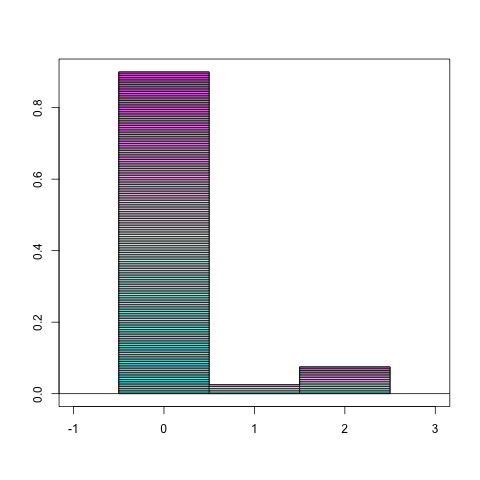
\includegraphics[width=12cm,height=10cm]{img/repProdB}
\end{center}


\item Il convient alors d'augmenter la taille d'échantillon et de sélectionner dans son nouveau échantillon les 50 premiers individus de son échantillon original. Qu'aurait-il pu en conclure~(rédaction standard)?

 
\IndicR
\begin{Verbatim}[frame=leftline,fontfamily=tt,fontshape=n,numbers=left]
> y50
 [1] 0 0 0 0 0 0 0 0 0 0 0 0 0 0 0 0 0 0 0 0 0 2 0 0 0 0 0 0 2 2 2 0 0 0 0 0 0 0
[39] 0 0 1 0 0 0 0 0 0 0 0 0
> mean(y50)
[1] 0.18
> # deltaEst.H0 <- (instruction R à fournir dans la rédaction)
> deltaEst.H0
[1] 0.3786397
\end{Verbatim}

 






\end{enumerate}

\noindent \underline{Partie~II}

En Janvier 2005, cela fait un an que le produit~B a été lancé. L'industriel pense que son produit mieux connu des consommateurs est plus vendu. Il dispose déjà de l'échantillon de taille $n=1000$ obtenu en 2004 (que l'on note ici \texttt{yB04}) ayant notamment servi à estimer le nombre moyen de produit~B vendus en 2004, désormais noté $\mu^{B04}$. En 2005, il décide d'interroger les mêmes $n=1000$ individus qu'en 2004. Le jeu de données associé est noté \texttt{yB05} servant notamment  à estimer le nombre moyen $\mu^{B05}$ de produit~B vendus en 2005.

\begin{enumerate}
\item Peut-on penser au vu de ces données qu'il y a eu une augmentation moyenne de 2004 à 2005 d'au moins $0.02$ en nombre de produit(s)~B vendu(s)~(rédaction standard)? 

\IndicR
\begin{Verbatim}[frame=leftline,fontfamily=tt,fontshape=n,numbers=left]
> yB05-yB04
   [1]  0  0  0  0  0  0  0  0  0  0  0  0  1  0  0  0  1  0  0  0  0 -2  0  0
  [25]  0  1  1  0 -2 -2 -2  0  0  0  0  0  0  0  0  0 -1  0  0  3  0  0  0  0
...
 [961]  0  0  0 -1  0  0  0  0  0  0  1  0  0  0  0  0  0  0 -1 -2  0  1  0  0
 [985]  0  0  0  0  3  1  0  0  0  0  0  0  0  0  0  0
> mean(yB05-yB04)
[1] 0.085
> # deltaEst.H0 <- (instruction R à fournir dans la rédaction)
> pnorm(deltaEst.H0)
[1] 0.991839
\end{Verbatim}

 




\item En fait, après réflexion, il réalise qu'il dispose  en 2005 de la valeur de $\mu^{B04}$ égale à $0.19$. Reformulez l'assertion d'intérêt et proposez l'instruction \texttt{R} fournissant la p-valeur associée.


\end{enumerate}

\noindent \underline{Partie~III}

Souhaitant exporter le produit~B en Allemagne, l'industriel se crée un échantillon de taille $n=500$ individus, consommateurs potentiels du produit~B allemands. Il souhaite alors comparer les deux pays. Ce nouveau jeu de données est noté \texttt{yAll}

On notera $\mu^{All}$ et $\sigma^2_{All}$ les moyennes et variances des réponses des consommateurs potentiels allemands. Pour simplifier, on notera $\mu^{Fr}$ et $\sigma^2_{Fr}$  les moyennes et variances des réponses des consommateurs potentiels français, et l'échantillon de taille 1000 est noté \texttt{yFr}. 

A partir des instructions \texttt{R} ci-dessous, combien d'assertions d'intérêt différentes (en précisant lesquelles) peut-on confirmer avec les données~?

\begin{Verbatim}[frame=leftline,fontfamily=tt,fontshape=n,numbers=left]
> (mean(yFr)-mean(yAll)-0.045)/seDMean(yFr,yAll)
[1] 1.821887
> pnorm((var(yFr)/var(yAll)-2)/seRVar(yFr,yAll))
[1] 0.996465
> pnorm((var(yAll)/var(yFr)-.5)/seRVar(yAll,yFr))
[1] 1.967895e-05
\end{Verbatim}



\end{exercice}






\end{document}


